% !TEX root = ../main.tex
% chktex-file 46
\chapter{Verwandte Arbeiten}%
\label{sec:related}

Das in~\ref{sec:intro:goals} beschriebene Ziel der automatisierten Wissensgraph-Konstruktion wird bereits seit langem erforscht.
Der Begriff \textit{Wissensgraph} wurde 2012 durch Google popularisiert, die Ideen dahinter lassen sich allerdings bis ins Ende des 19. Jahrhunderts zurückverfolgen.
Dieses Kapitel zeigt auf, wie sich die Themen dieser Arbeit in die bisherige Forschung einfügen.
\ref{sec:related:kr} ordnet hierfür das Konzept des Wissensgraphen in die Entwicklungsgeschichte der Wissensrepräsentation ein. % chktex 2
In~\ref{sec:related:nlp} wird ein Überblick über die momentan verbreiteten \textit{Natural Language Processing} (NLP) Werkzeuge gegeben.
Das Wissensgraphkonzept und NLP wird schließlich in~\ref{sec:related:kgc} kombiniert und es werden die aktuell verwendeten Verfahren zur Wissensgraph-Konstruktion beschrieben.

\section{Ansätze zur Wissensrepräsentation}%
\label{sec:related:kr}

\subsection{Logische Grundlagen}%
\label{sec:related:kr:logic}

Die Entwicklung der Wissensrepräsentation hängt eng mit der Entwicklung der Logik zusammen.
Während in der formalen Logik und Mathematik die Prädikatenlogik das allgemein verwendete Kalkül ist und alternative Formalismen kaum verbreitet sind, finden im Bereich der Wissensrepräsentation bis heute diverse andere Kalküle Verwendung.
Diese werden im Folgenden kurz vorgestellt.

\paragraph{Begriffsschrift (1879)}
Gottlob Freges Buch über die \textit{Begriffsschrift}~\cite{Frege1879} gilt als eines der bedeutsamsten Werke der Logik.
Sie ist der erste Formalismus mit der Ausdrucksstärke der modernen Prädikatenlogik zweiter Ordnung mit Identität.
Frege benutzt hierfür eine zweidimensionale Notation, die sich stark von der heute gebräuchlichen linearen, an die Algebra angelehnten Notation unterscheidet.
\begin{equation*}
	\vcenter{\hbox{\Fconditional[\Fanqn{a}]{\Fcontent \mathfrak{R(a)}}{\Fncontent \mathfrak{P(a)}}}}
	\quad\Leftrightarrow\quad
	\exists\ a: P(a) \lor R(a)
\end{equation*}
Im Gegensatz zur Prädikatenlogik gibt es keine eigene Syntax für \textit{UND} und \textit{ODER};
diese Operatoren müssen durch die Kombination von Negation und Implikation abgebildet werden.
Zudem gibt es ausschließlich den Allquantor;
eine existenzquantisierte Aussage muss durch Negation der negierten allquantisierten Aussage ausgedrückt werden.

\paragraph{Prädikatenlogik: Peirce Notation (1885)}
Unabhängig von Frege entwickelte der amerikanische Mathematiker Charles Sanders Peirce ebenfalls ein prädikatenlogisches Kalkül~\cite{Peirce1885}.
Peirces Notation hatte starke Ähnlichkeiten mit der heute benutzten linearen Schreibweise.
Statt den modernen Symbolen hat Peirce allerdings die algebraischen Operatoren benutzt, um die Analogien zwischen Logik und Algebra auszudrücken.
\begin{equation*}
	\Sigma_a\ P_a + R_a
	\quad\Leftrightarrow\quad
	\exists\ a: P(a) \lor R(a)
\end{equation*}

\paragraph{Existential Graphs (1897)}
Neben seiner zuvor entwickelten linearen prädikatenlogischen Notation, hat Peirce zudem viele Jahre an einem alternativen graphischen Kalkül gearbeitet, welches er \textit{Existential Graphs} (zu dt.~Existenzgraphen)~\cite{Sowa2011} nannte.
Ähnlich wie die Begriffsschrift werden Existenzgraphen zweidimensional dargestellt.
Von dieser Gemeinsamkeit abgesehen, funktionieren sie allerdings fundamental verschieden.
Ein logischer Ausdruck wird hier durch einen ungerichteten Graphen beschrieben.
Die konkrete räumliche Anordnung der Knoten und Kanten hat dabei keine semantische Relevanz.

Peirce hat Existenzgraphen als ein dreistufiges aufeinander aufbauendes System konzipiert.
Die erste Stufe, die sog.\ $\alpha$-Graphen, umfasst alle notwendigen syntaktischen Elemente, um ein Kalkül mit der Ausdrucksstärke der Aussagenlogik zu erhalten.
Die $\beta$-Graphen bilden die zweite Stufe und erweitern die Syntax der $\alpha$-Graphen, sodass die Ausdrucksstärke der Prädikatenlogik erster Ordnung erreicht wird.
Sowohl für $\alpha$- als auch für $\beta$-Graphen ist die Vollständigkeit und Korrektheit bewiesen.
Die dritte Stufe ($\gamma$-Graphen) wurde von Pierce nie vollendet;
sie deckt in etwa die Ausdrucksstärke der heutigen Prädikatenlogik höherer Ordnung sowie der Modallogik ab.
\begin{align*}
	\vcenter{\hbox{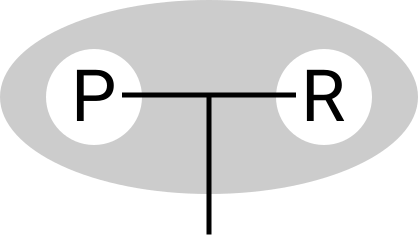
\includegraphics[height=3em]{gfx/related-work/existentialGraphExample1.pdf}}}
	\quad\Leftrightarrow\quad
	\exists\ a: P(a) \lor R(a)
\end{align*}
Wie schon die Begriffsschrift, sind Existenzgraphen syntaktisch minimal.
Direkt ausdrücken lässt sich lediglich \textit{UND}, der Existenzquantor und die Negation.
Ein weiterer Unterschied zur heutigen Prädikatenlogik ist die Beschreibung logischer Inferenzen.
Im Gegensatz zu den prädikatenlogischen Ersetzungsaxiomen, die auf der syntaktischen Struktur von logischen Ausdrücken operieren (z.~B. für Kommutativität), lassen sich die Ersetzungsaxiome für Existenzgraphen als Graphtransformationsregeln verstehen, die bestimmte Teilmengen der Knoten und Kanten eines Ausdrucks durch andere äquivalente Knoten- und Kantenmengen ersetzen.

\paragraph{Prädikatenlogik: Peano-Russell Notation (1910)}
Die zweidimensionalen Notationen wurde häufig kritisiert, da sie die lineare, algebraische Notation der symbolischen Logik von Boole und De Morgan verwarfen~\cite{Sluga1987}.
Freges Begriffsschrift und Peirces Existenzgraphen konnten sich daher nicht durchsetzen.
Peirces algebraische prädikatenlogische Notation hingegen, stieß auf größere Akzeptanz.
Giuseppe Peano hat auf deren Basis eine ähnliche Notation entwickelt, welche allerdings nicht die algebraischen Operatoren benutzt, damit sich logische Ausdrücke besser mit mathematischen Ausdrücken kombinieren lassen.
Bertrand Russell hat Peanos Notation anschließend in leicht abgewandelter Form in den \textit{Principia Mathematica}~\cite{Whitehead1910} benutzt.
Diese sog.~Peano-Russell-Notation ist im Wesentlichen identisch mit der modernen Schreibweise.

Trotz des Verschwindens der zweidimensionalen Notationen, finden sich noch heute Anlehnungen daran~\cite{Begriffsschrift}.
So ist z.~B. die Negation $\lnot A$ auf Freges negierten Inhaltsstrich $\Fncontent A$ und der Ableitungsoperator $\vdash$ auf Freges Urteilsstrich mit angefügtem Inhaltsstrich $\Facontent$ zurückzuführen.

\subsection{Entwicklung maschineller Wissensrepräsentation}%
\label{sec:related:kr:history}

Die Idee, Computer zur Lösung beliebiger Probleme zu benutzen, ist nicht neu.
Da ein solches maschinelles Problemlösen die Verfügbarkeit von Hintergrundwissen über die Problemdomäne erfordert,
wurden Methoden zur Wissensrepräsentation immer im Zusammenhang mit Problemlösern erforscht~\cite{Hayes-Roth1983}.
So wie effiziente Datenstrukturen die Implementation effizienter Algorithmen ermöglichen, ermöglichen gute Wissensrepräsentationen die Implementation guter Problemlöser.
Was genau nun als ein guter Problemlöser verstanden wird, hat sich im Laufe der Jahre allerdings immer wieder verändert.

\paragraph{Universelle Problemlöser}
Einer der ersten maschinellen Problemlöser war der von Newell und Simon 1955 entwickelte \textit{Logic Theorist} (LT)~\cite{Newell1956}.
LT war in der Lage logische Aussagen zu beweisen, indem er systematisch Ersetzungsaxiome auf eine gegebene Aussage angewandt hat, bis die gesuchte Lösung abgeleitet wurde.

Die Grundidee des LT haben Newell, Simon und Shaw 1959 im \textit{General Problem Solver} (GPS)~\cite{Newell1959} erweitert.
Es wurden Heuristiken hinzugefügt, um den Suchraum geschickter zu durchlaufen.
GPS war ein universeller Problemlöser, konnte also jedes Problem lösen, das sich durch eine Menge von Horn-Klauseln ausdrücken lässt.
Zwar war es so theoretisch möglich Probleme aus diversen Domänen zu lösen, aufgrund der kombinatorischen Explosion war GPS alledings nicht zur Lösung komplexer praktischer Probleme geeignet.

\paragraph{Expertensysteme}
Aufgrund der Misserfolge universeller Problemlöser für praktische Probleme hat die Forschung begonnen, sich mehr auf die Entwicklung von Expertensystemen zu fokussieren.
Expertensysteme besitzen für gewöhnlich eine Wissensbasis, in der domänenspezifisches Wissen in Form von Regeln und Fakten kodiert ist.
Eine sog.~Inferenzmaschine benutzt diese Regeln und Fakten um Probleme zu lösen.

\paragraph{Semantic Networks (1956)}
Die Idee, Graphen als Datenstruktur für Wissensbasen zu verwenden, taucht im Kontext der Informatik erstmals unter dem Begriff \textit{Semantic Networks}~\cite{Lehmann1992} (zu dt.~semantische Netzwerke) auf.
Dieser Ansatz beschreibt Wissen als Menge von $(subject,\allowbreak predicate,\allowbreak object)$-Tripeln.
Es gibt darüber hinaus allerdings keine klaren Regeln, wie ein semantisches Netz strukturiert sein muss.
Semantische Netzwerke sind daher primär als ein Oberbegriff für die große Vielfalt konkreter graphbasierter Wissensbasen zu verstehen.
Dennoch lässt sich eine Gemeinsamkeit zwischen den diversen Ansätze festmachen:
Meist kommt die sog.\ \textit{IS-A}-Relation vor~\cite{Brachman1983}, welche das Konzept der Vererbung repräsentiert.
Die Beschreibung von baumartigen Taxonomien mittels \textit{IS-A} ist ein häufiges Einsatzgebiet semantischer Netzwerke.

\paragraph{Conceptual Graphs (1976)}
Wie genau mit Graphen komplexes Wissen beschrieben werden kann, das über eine reine Taxonomie hinaus geht, blieb bei semantischen Netzen unklar.
John F. Sowas \textit{Conceptual Graphs}~\cite{Sowa1976}\cite{Harmelen2007} (zu dt.~Konzeptgraphen) lösen dieses Problem.
Statt Wissen lediglich als eine einfache Menge von Beziehungen abzubilden, wird es als prädikatenlogischer Ausdruck verstanden.
Hierfür baut Sowa auf Peirces Existenzgraphen auf, die bis dahin weitestgehend unbeachtet waren.
\begin{align*}
	\vcenter{\hbox{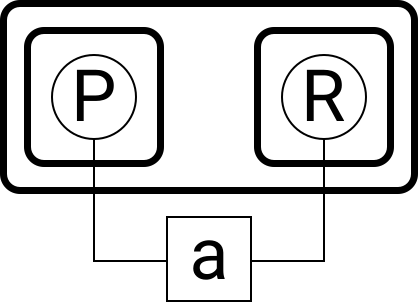
\includegraphics[height=4em]{gfx/related-work/conceptGraphExample1.pdf}}}
	\quad\Leftrightarrow\quad
	\exists\ a: P(a) \lor R(a)
\end{align*}
Dieser Ansatz erlaubt es komplexe Wissensbasen zu konstruieren, in denen nicht nur gespeichert werden kann, ob ein Konzept existiert, sondern auch, ob es nicht oder nur möglicherweise existiert.
Da Konzeptgraphen, so wie schon die Existenzgraphen, ein vollständiges und korrektes Logikkalkül sind, lassen sich zudem Inferenzregeln für sie definieren.
Der Vorteil hierfür einen Graphen statt eines prädikatenlogischen Ausdrucks zu verwenden ist, dass eine Graphstruktur einen deutlich effizienteren Zugriff auf gespeichertes Wissen ermöglicht.

\paragraph{Knowledge Graphs (1987)}
Der Begriff \textit{Knowledge Graph}~\cite{Riet1992} (zu dt.~Wissensgraph) bezeichnete ursprünglich eine Klasse semantischer Netze, deren Relationsmenge formal spezifiziert ist.
Die Menge erlaubter Graphen wird hierdurch so eingeschränkt, dass das repräsentierte Wissen eindeutig interpretierbar und ohne Redundanz ist.
Dies erlaubt die Definition von Inferenzregeln, um Schlussfolgerungen aus einem gegebenen Graphen zu ziehen.
Im Laufe der Jahre ist die Grenze zwischen semantischen Netzen und Wissensgraphen allerdings so stark verschwommen, dass heute auch mehrdeutige, redundanzbehaftete semantische Netze, die lediglich wenige Relationstypen benutzen, als Wissensgraphen bezeichnet werden~\cite{McCusker2016}.
Wissensgraphen und Konzeptgraphen müssen weiterhin streng unterschieden werden, da erstere oftmals Negation und Modalität nicht unterstützen.

\subsection{Aktuelle Wissensrepräsentationsprojekte}%
\label{sec:related:kr:today}

\subsubsection{Manuelle Ansätze}

\paragraph{Semantic Web}
Das sog.~\textit{Semantic Web} bezeichnet eine Menge von W3C-Standards, die das bestehende Web um eine formale Wissensbeschreibungssyntax erweitern~\cite{SemWeb}.
Zentral ist dabei das \textit{Resource Description Framework} (RDF), mit dem sich beliebige Konzepte, auch Ressourcen genannt, beschreiben und verknüpfen lassen.
Ziel ist es, über die unstrukturierte Netzstruktur des bestehenden Webs, eine strukturierte, leicht maschinell verarbeitbare Netzstruktur zu legen.
Durch die Anfragesprache \textit{SPARQL} ist es möglich, Wissen aus diesem Netz auszulesen.
Das Web würde somit zu einem großen denzentralen Wissensgraphen.
Tim Berners-Lee beschreibt diese Idee als das ``Web 3.0''~\cite{Shannon2006}.
Obwohl die Technologien hierfür bereits seit Jahren existieren, sind bislang nur wenige Webseiten mit RDF-Tags annotiert.
Häufige Kritik ist, dass das Semantic Web zu viel theoretisches Hintergrundwissen über Wissensrepräsentationsverfahren erfordert, um für die meisten Webseitenbetreiber zugänglich zu sein~\cite{Marshall2003}.

\paragraph{WordNet}
Das \textit{WordNet} der Universität Princeton~\cite{WordNet} ist ein frei verfügbares lexikalisch-semantisches Netz für die englische Sprache, d.~h.\ ein semantisches Netz, welches die Bedeutung von Worten in Relation zueinander setzt.
Relationen werden dabei z.~B. für Synonyme, Hypernyme (Oberbegriffe) und Meronyme (Bestandteile) eingefügt.
Der Datenbestand des WordNets wird manuell gepflegt und resultiert aus der Kombination der Einträge verschiedener Wörterbücher.

\subsubsection{Automatisierte Ansätze}
Neben den manuellen Grapherzeugungsansätzen des Semantic Webs und des WordNets gibt es diverse voll- und semiautomatische Ansätze.
Diese bauen die Graphstruktur selbstständig aus gegebenen Datenquellen auf.

\paragraph{NELL}
Das \textit{Never-Ending Language Learning} (NELL) System~\cite{Carlson2010} traversiert selbstständig das Internet und fügt die gefundenen textuellen Informationen in einen Wissensgraphen ein.
Hierfür wird eine Kombination verschiedener Modelle verwendet, die regelmäßig angepasst wird.
Menschen können optional Feedback für die extrahierten Fakten geben, um die Inferenzqualität weiter zu verbessern.

\paragraph{Google Knowledge Graph}
Basierend auf den Ideen der in~\ref{sec:related:kr:history} vorgestellten Wissensgraphen, stellte Google 2012 eine eigene, ebenfalls \textit{Knowledge Graph} genannte, Wissensgraphtechnologie vor~\cite{Singhal2012}.
Sie wird benutzt, um Suchanfragen semantisch statt per String-Matching zu beantworten.
So können z.~B. zum Suchbegriff verwandte Ergebnisse angezeigt werden, selbst wenn es keine textuelle Ähnlichkeit zu jenem gibt.
Laut Googles Aussagen stammen die Quelldaten u.~a.\ aus Wikipedia Infoboxen, Wikidata und dem CIA World Factbook.
Da es sich hierbei, im Gegensatz zu NELL, primär um strukturierte Daten handelt, ist das automatisierte Einpflegen mit hoher Genauigkeit möglich.
Mit welcher Ontologie die Daten im Graph repräsentiert werden und wie sie in diese Repräsentation übersetzt werden, ist nicht öffentlich bekannt.
Obwohl bislang nur wenig über die Technologie veröffentlicht wurde, lässt sich beobachten, dass das öffentliche Interesse an der Thematik seit Googles Ankündigung im Mai 2012 deutlich gestiegen ist~\fref{fig:related:kgTrend}.

\begin{figure}[h]
	\centering
	\begin{tikzpicture}
		\pgfplotstableread[col sep=comma] {data/related-work/knowledgeGraph.csv}\knowledgeGraphTrend%
		\begin{axis}[
			width=0.8\textwidth,
			height=5cm,
			smooth,
			axis x line=bottom,
			axis line style={draw=none},
			ytick style={draw=none},
			ymin=0,
			ymax=100,
			ymajorgrids,
			ylabel={Popularität in \%},
			date coordinates in=x,
			date ZERO=2004-01-01,
			xmin={2004-01-01},
			xmax={2017-08-01},
			xticklabel={\month.\year},
			xtick={2004-01-01,2012-05-01,2017-08-01}
		]
			\addplot+[no markers,style=thick] table [x=month, y=popularity]{\knowledgeGraphTrend};
		\end{axis}
	\end{tikzpicture}
	\caption{Popularität des Begriffs ``knowledge graph'' (Quelle: Google Trends~\cite{Google2017})}\label{fig:related:kgTrend}
\end{figure}

\section{NLP-Werkzeuge}%
\label{sec:related:nlp}

Neben der Repräsentation von Wissen, ist auch die Verarbeitung natürlicher Sprache eine Kernaufgabe dieser Arbeit.
Hierfür existiert bereits eine Vielzahl von \textit{Natural Language Processing} (NLP) Werkzeugen.
Trotz dieser Vielfalt lassen sich grundlegende Verarbeitungsschritte festmachen, die in den meisten Werkeugen verwendet werden.
\begin{enumerate}
	\item \textbf{Tokenization:}
		In der Regel einer der ersten Verarbeitungsschritte einer NLP Bibliothek.
		Eine Eingabezeichenkette wird dabei in eine Liste von Token zerlegt.
		Token sind u.~a. Wörter, Satzzeichen und numerische Literale.
		\[
			\text{``Today I'm testing myself.''}
			\rightarrow
			(\text{Today}, \text{I}, \text{'m}, \text{testing}, \text{myself}, \text{.})
		\]
	\item \textbf{Lemmatization:}
		Abbildung von Token auf ihre Lemmata (Grundformen).
		\[
			(\text{Today}, \text{I}, \text{'m}, \text{testing}, \text{myself}, \text{.})
			\rightarrow
			(\text {today}, \text{I}, \text{be}, \text{test}, \text{myself}, \text{.})
		\]
	\item \textbf{Part-of-speech Tagging:}
		Abbildung von Token auf ihre Wortarten und Flexionen (POS-Tags).
		\begin{center}
			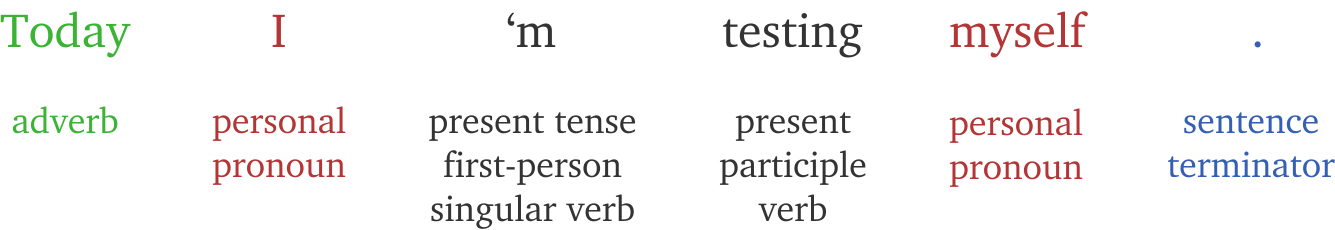
\includegraphics[height=4.5em]{gfx/related-work/posTaggingExample1.pdf}
		\end{center}
	\item \textbf{Named Entity Recognition:}
		Klassifizierung von Token in Kategorien wie z.~B. Person, Ort oder Zeitpunkt.
		\[
			({\color{gruen}\underbrace{\text{Today}}_{\text{date}}}, \text{I}, \text{'m}, \text{testing}, \text{myself}, \text{.})
		\]
	\item \textbf{Coreference Resolution:}
		Bestimmung von Token-Äquivalenzklassen, die jeweils auf dasselbe Konzept verweisen (insbesondere Pronomina und ihr Antezedens).
		\begin{align*}
			(\text{Today}, \tikzmark{a}\text{\color{rot}I}, \text{'m},
			 \text{testing}, \text{\color{rot}mys}\tikzmark{b}\text{\color{rot}elf}, \text{.})
			\begin{tikzpicture}[overlay,remember picture]
				\draw[-,rot,shorten >=3pt,shorten <=3pt] (a.center) to[bend right] (b.center);
			\end{tikzpicture}
		\end{align*}
	\item \textbf{Dependency Parsing:}
		Eine auf den Part-of-speech-Tags aufbauende syntaktische Analyse, welche die grammatikalischen Abhängigkeiten der Token untereinander ausgibt.
		Die Menge dieser Abhängigkeiten bildet einen Baum oder baumähnlichen Graphen, der \textit{Treebank} bzw.\ \textit{Dependency Graph} genannt wird.
		\begin{center}
			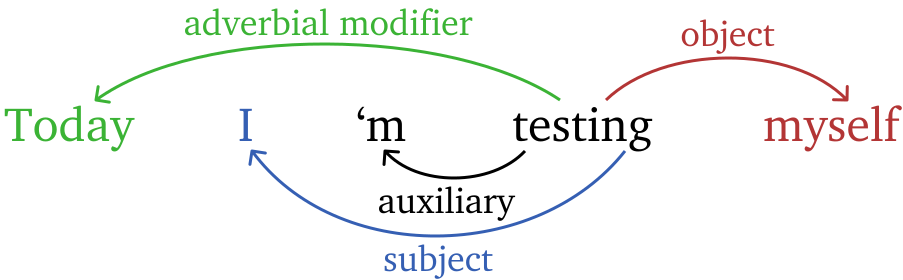
\includegraphics[height=5.5em]{gfx/related-work/depParseExample1.pdf}
		\end{center}
\end{enumerate}

Wie sich erkennen lässt, bauen die Verarbeitungsschritte sukzessive aufeinander auf und bilden eine Art Pipeline~\cite{Pipeline}.
Dieses Pipeline-Modell findet sich in vielen NLP-Werkzeugen wieder.
Ein solches Werkzeug ist z.~B. das quelloffene Stanford~CoreNLP Projekt~\cite{Manning2014}\cite{CoreNLP}, welches u.~a. Module für alle der soeben vorgestellten Verarbeitungsschritte beinhaltet.
Ein alternatives NLP-Toolkit ist Apache~OpenNLP~\cite{OpenNLP};\@
es bietet ähnliche Module wie CoreNLP an.

\section{Wissensgraph-Konstruktionsverfahren}%
\label{sec:related:kgc}

Wie in~\ref{sec:related:kr:today} gezeigt, gibt es diverse Ansätze um Graphen aus Daten zu konstruieren.
Da für das Thema dieser Arbeit insbesondere automatisierte Verfahren relevant sind, die mit unstrukurierten Daten, wie z.~B. natürlicher Sprache, umgehen können, werden diese im Folgenden näher beschrieben.

Üblicherweise arbeiten Wissensgraph-Konstruktionsverfahren nicht direkt mit den unstrukturierten Eingabedaten, wie z.~B. den Inhalten von E-Mails,
sondern mit einer Knoten- bzw.\ Konzeptmenge und ggf.\ auch einer Kanten- bzw.\ Relationsmenge, die zuvor, z.~B. mittels eines in~\ref{sec:related:nlp} vorgestellten NLP-Verfahrens, aus den Rohdaten extrahiert wurden.
Die Wissensgraph-Konstruktion ist somit äquivalent zum Problem der \textit{Link Prediction}, also dem Finden von Relationen zwischen den gegebenen Konzepten.
Die Link Prediction wiederum lässt sich als ein Problem des \textit{Statistical Relational Learnings} (SRL) auffassen.
In der Literatur finden sich im Wesentlichen drei Klassen von SRL-Verfahren~\cite{Nickel2016}, die auf verschiedenen Annahmen über die Korrelation der zu verknüpfenden Informationen basieren:
\begin{enumerate}
	\item \textbf{Latent Feature Models:}
		Alle Relationen werden als bedingt unabhängig angenommen, sofern bestimmte Eigenschaften über Subjekte und Objekte der Relationen gegeben sind.
	\item \textbf{Graph Feature Models:}
		Alle Relationen werden als bedingt unabhängig angenommen, sofern bestimmte Eigenschaften der Struktur des Graphen gegeben sind.
	\item \textbf{Markov Random Fields:}
		Es wird angenommen und erlaubt, dass alle Relationen lokale Abhängigkeiten voneinander haben können.
\end{enumerate}

\paragraph{Latent Feature Models}
Ein Beispiel für ein Latent-Feature-Modell ist das RESCAL-Verfahren~\cite{Nickel2013}, welches auf Tensorfaktorisierung basiert.
Die Grundidee dabei ist es, allen Entitäten $i$ einen Vektor $e_i \in \mathbb{R}^H$, welcher $H$ Eigenschaften bzw.\ Features von $i$ repräsentiert, zuzuordnen und für alle Relationen $k$ eine Gewichtsmatrix $W_k \in \mathbb{R}^{H \times H}$ zu finden.
Die Konfidenz in die Existenz einer Relation $i \xrightarrow{k} j$ wird durch $e_i^\top\ W_k\ e_j$ beschrieben.
Diese Definition ermöglicht eine sehr schnelle Link Prediction, da lediglich ein Vektor-Matrix-Vektor-Produkt berechnet werden muss.
RESCAL liefert gute Ergebnisse, wenn die vorherzusagenden Relationen globale Abhängigkeiten aufweisen.
Lokal stark zusammenhängende Teilgraphen werden allerdings schlecht erkannt, da nur der Feature-Vektor und nicht die Nachbarschaft einer Entität berücksichtigt wird;
ein Beispiel hierfür sind symmetrische Relationen.
\[A \xrightarrow{\text{married to}} B \implies B \xrightarrow{\text{married to}} A\]

\paragraph{Graph Feature Models}
Komplementär zu den Latent-Feature-Modellen sind die Graph-Feature-Modelle.
Statt Entitäten in einen Feature-Raum einzubetten, wird hier die Nachbarschaft der Entitäten betrachtet.
Ein Beispiel hierfür ist der \textit{Path Ranking Algorithmus} (PRA)~\cite{Lao2011}. PRA ermittelt Relationen durch zufälliges Durchwandern des Graphen.
Um die Stärken der Latent Feature und Graph-Feature-Modelle zu kombinieren, wurden Hybrid-Modelle, wie z.~B. das \textit{Additive Relational Effects} (ARE) Verfahren~\cite{Nickel2014}, entwickelt, welches die Konfidenzen von RESCAL und PRA addiert.

\paragraph{Markov Random Fields}
Fundamental verschieden von diesen beiden Verfahren sind \textit{Markov Random Fields} (MRFs).
Hier sind prinzipiell Abhängigkeiten zwischen allen Relationen möglich, was MRFs sehr flexibel macht.
Da dies hinsichtlich der Laufzeit schnell impraktikabel wird, wird das Modell um einen Abhängigkeitsgraphen erweitert, der die Anzahl von betrachteten Abhängigkeiten reduziert.
Der Abhängigkeitsgraph darf dabei nicht mit dem Wissensgraphen verwechselt werden:
Der Abhängigkeitsgraph beschreibt statistische Abhängigkeiten zwischen Relationen, während der Wissensgraph Relationen zwischen Konzepten beschreibt.
Zur Modellierung von Abhängigkeitsgraphen werden i.~d.~R. Kalküle verwendet, die an eine Prädikatenlogik erster Ordnung angelehnt sind.
Das Finden eines Wissensgraphen ist in diesem Modell analog zum Lösen des MAX-SAT-Problems.
Wählt man ein Kalkül, in dem die Atome (i.~e.\ Zufallsvariablen des MRFs) aus $[0, 1]$ sind und Formeln zudem ausschließlich Disjunktionen und Negationen gemäß Łukasiewicz T-Norm enthalten, erhält man ein sog.\ \textit{Hinge-Loss-MRF}~\cite{Bach2013}\cite{Bach2015}.

Ein konkretes Kalkül, welches sich zur Spezifikation von HL-MRFs eignet, ist die \textit{Probabilistic Soft Logic} (PSL)~\cite{Broecheler2010}\cite{Bach2015}.
MAX-SAT lässt sich für solche HL-MRFs effizient und parallelisierbar mit dem konvexen \textit{Alternating Direction Method of Multipliers} (ADMM) Optimierungsverfahren~\cite{Boyd2011} lösen.
In seiner ursprünglichen Form ist ADMM allerdings ausschließlich für offline Inferenz geeignet;
der Wissensgraph müsste also bei jeder Eingabe neu konstruiert werden.
Um dieses Problem zu lösen, wurde das \textit{Budgeted Online Collective Inference} (BOCI) Verfahren~\cite{Pujara2015} entwickelt.
BOCI nutzt Metadaten, die während der Ausführung von ADMM anfallen, um eine Bewertung für jedes Atom zu berechnen.
Die Bewertung eines Atoms beschreibt, wie groß die erwartete Wertveränderung beim Eintreffen neuer Informationen ist.
Kommen nun neue Informationen an, müssen ausschließlich die $m$ höchstbewerteten Atome betrachtet werden, die Werte aller anderen Atome werden fixiert.
Je höher das Budget $m$, desto höher ist die Qualität im Vergleich zu einer Neukonstruktion des Graphen.
Es wurde empirisch gezeigt, dass die Inferenzqualität mit BOCI oft nur unwesentlich schlechter ist als bei einer kompletten Offline-Inferenz.

Die Kombination von PSL, ADMM und BOCI ist daher ein guter Ausgangspunkt für den Entwurf eines Online-Wissensgraph-Konstruktionsverfahrens.
Der Vorteil dieses Ansatzes gegenüber Latent-Feature- oder Graph-Feature-Modellen ist, dass sich domänenspezifische Expertensysteme, z.~B. Geoinformationssysteme, leicht in eine PSL-Inferenz integrieren lassen.
PSL erlaubt nämlich die Inklusion von benutzerdefinierten Funktionen und Prädikaten.
Diese können benutzt werden, um z.~B. die Levenshtein-Distanz zweier Zeichenketten oder domänenspezifisches Hintergrundwissen, wie die Distanz zwischen zwei namentlich genannten Orten, mit in die Entity Resolution einfließen zu lassen.
